\documentclass[handout]{beamer}
\usepackage{graphicx}
\usepackage{dirtytalk}
\usepackage{hyperref}
\usetheme{Antibes}
\title{CS419 Project \\ Exploring GANs and Application\footnote{\href{https://github.com/siddhant-midha/CS419M-Project}{\texttt{https://github.com/siddhant-midha/CS419M-Project}}}}
%https://github.com/siddhant-midha/CS419M-Project
\author{}
\date{}
\usepackage{mathtools}
\usepackage{physics}
\usepackage{float}
\newcommand{\R}{\mathbb{R}}
\newcommand{\Z}{\mathbb{Z}}
\newcommand{\T}{\mathbb{T}}
\newcommand{\E}{\mathbb{E}}
\newcommand{\p}{\mathbb{P}}
\newcommand{\N}{\mathbb{N}}
\newcommand{\C}{\mathbb{C}}
\newcommand{\K}{\mathbb{K}}
\newcommand{\w}{\wedge}
\usepackage{tikz}
\begin{document}
\frame{\titlepage}
%=================
\AtBeginSection[]
{\begin{frame}
\frametitle{Table of Contents}
\tableofcontents
\end{frame}}
%==================
\section{Introduction}
\begin{frame}{Motivation}
    \begin{itemize}
        \item Throughout the course, we were exposed to a variety of algorithms and basic ML techniques. \pause
        \item We were also briefly introduced to deep learning.\pause
        \item Hence, we took up this project to help us appreciate some crucial aspects of deep learning all the while understanding the fundamentals.\pause
        \item Out of interest, we opted for GANs.\pause
        \item Out of more interest, we chose image translation -- particularly, anime face colouration.\pause

    \end{itemize}
\end{frame}
\section{GAN?}
\begin{frame}{What are GANs?}
    \begin{itemize}
        \item TLDR: GANs implicitly estimate distributions by learning the ability to sample from them.\pause
        \item Two components,\pause
        \begin{enumerate}
            \item Generator (G) -- The artist: Tries to generate samples from the distribution.\pause
            \item Discriminator (D) -- The art critic:  Tries to root out generated samples from the real samples. \pause
        \end{enumerate}
        \item This competition enables the learning of a mapping from the latent space to the image space.\pause
    \end{itemize}
\end{frame}
\begin{frame}{What are GANs?}
Formally, we have\pause
\[J_D(\theta_D,\theta_G) := -(\mathbb{E}_{x \sim p_{data}}log(D(x)) +\mathbb{E}_zlog(1 - D(G(z))))\]\pause
\[J_G(\theta_D,\theta_G) := -J_D(\theta_D,\theta_G)\]\pause
Define $V(\theta_D,\theta_G) := -J_D(\theta_D,\theta_G)$. \pause Thus we have the following game \pause
\[\min_{\theta_G}\max_{\theta_D}V(\theta_G,\theta_D)\]\pause
Minima achieved when $G$ draws samples exactly from the distribution.
\end{frame}
\section{Work Done}
\begin{frame}{A basic GAN}
\begin{itemize}
    \item We observed that the $G$ and $D$ functions incur a lot of freedom in design.\pause
    \item Hence, we began with a basic design wherein both of them consist of Dense layers.\pause 
    \item We noted that certain up sampling is required in the $G$ architecture.\pause
    \item Also noted that down sampling is needed in the $D$ architecture, followed by a $\texttt{sigmoid}$. \pause
    \item We trained this basic GAN on both \texttt{MNIST} and \texttt{Fashion-MNIST} datasets.
    
\end{itemize}
\end{frame}
\begin{frame}{A basic GAN -- Results}
    
    \begin{figure}[H]
        \centering
        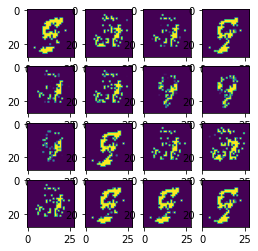
\includegraphics[height = 6cm, width = 6cm]{2nd_attempt_mnist_20epoc.png}
        \caption{MNIST, 20 epochs}
        \label{fig:my_label}
    \end{figure}
\end{frame}
\begin{frame}{A basic GAN -- Results}
    
    \begin{figure}[H]
        \centering
        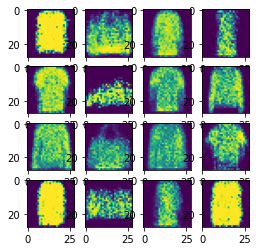
\includegraphics[height = 6cm, width = 6cm]{on_f_mnist.png}
        \caption{FashionMNIST, 20 epochs}
        \label{fig:my_label}
    \end{figure}
\end{frame}
\begin{frame}{A basic GAN -- Observations}
    \begin{itemize}
        \item We see that overall performance is better on the \texttt{Fashion-MNIST} dataset.\pause
        \item Even more so, we note that additional batch normalization was needed in order for the GAN to work on the \texttt{MNIST} dataset. \pause
        \item That is, initially the exact same model performed much better on the former than the latter -- intricacies in the dataset.\pause
    \end{itemize}
\end{frame}
\begin{frame}{A deeper GAN}
\begin{itemize}

    \item We note the deficiencies in the basic GAN architecture, and realize the need for convolutional layers to preserve local information in images.\pause
    \item Here we implement the convolutional-GAN.
    \item We implement this on \texttt{MNIST} and \texttt{FashionMNIST} datasets.\pause
    \end{itemize}
\end{frame}
\begin{frame}{A deeper GAN -- Results}
    \begin{figure}[H]
        \centering
        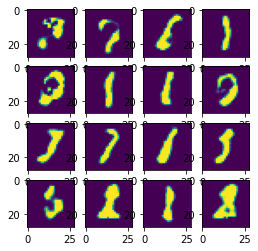
\includegraphics[height = 6cm, width = 6cm]{convGAN_MNIST_20epoc.png}
        \caption{MNIST, 20 epochs}
        \label{fig:my_label}
    \end{figure}
\end{frame}
\begin{frame}{A deeper GAN -- Results}
    \begin{figure}[H]
        \centering
        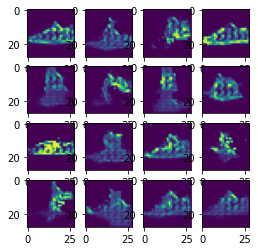
\includegraphics[height = 6cm, width = 6cm]{convGAN_FashionMNIST_50epoc_LESSBNORM (nice).png}
        \caption{FashionMNIST, 50 epochs}
        \label{fig:my_label}
    \end{figure}
\end{frame}
\begin{frame}{A deeper GAN -- observations}
    \begin{itemize}
    \item Image quality improves, as expected.\pause
        \item Surprisingly, here with batchnorm and 20 epochs.\pause \texttt{MNIST} does much better than \texttt{FashionMNIST}.
        \item Then, we try increasing the number of epochs for the former. \pause
        \item Does not help.\pause
        \item Decreasing Batchnorm helps.
    \end{itemize}
\end{frame}
\begin{frame}{Conditioning the GAN}
\begin{itemize}

    \item We appreciate the use of GANs for sampling from distributions.\pause
    \item We now require to sample from particular classes.\pause
    \item That is, we feed the class-labels (such as the digit \texttt{7} in \texttt{MNIST}) in the training process.\pause
    \item Hence getting conditional-GAN.
    \end{itemize}
\end{frame}
\begin{frame}{Conditoning the GAN -- Results}
    \begin{figure}[H]
        \centering
        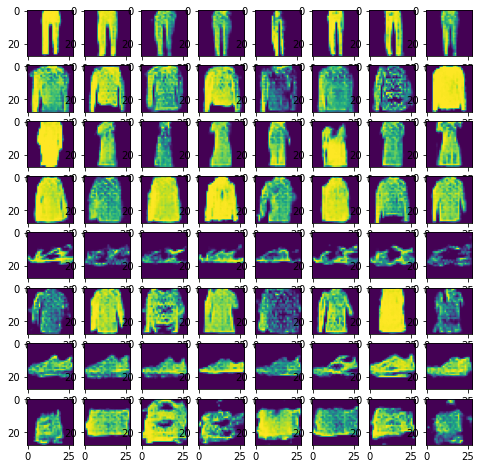
\includegraphics[height = 6cm, width = 6cm]{condGAN_Fashion_20epoc.png}
        \caption{FashionMNIST, 20 epochs, each row corr. to one class query}
        \label{fig:my_label}
    \end{figure}
\end{frame}
\begin{frame}{Conditoning the GAN -- Results}
      \begin{figure}[H]
        \centering
        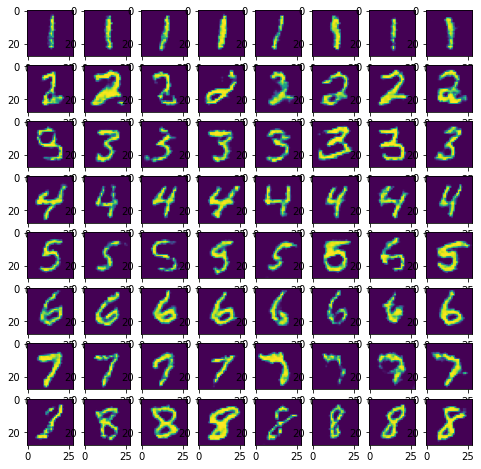
\includegraphics[height = 6cm, width = 6cm]{condGAN_MNIST_20epoc.png}
        \caption{MNIST, 20 epochs, each row corr. to one class query}
        \label{fig:my_label}
    \end{figure}
\end{frame}
\begin{frame}{Conditioning the GAN -- Observations}
    \begin{itemize}
        \item We had to modify the architecture in code due to taking class label as input -- explained in report. \pause 
        \item \texttt{FashionMNIST} trained faster than \texttt{MNIST}. \pause
        \item We did not require additional batchnorm for \texttt{MNIST}.
    \end{itemize}
\end{frame}
\begin{frame}{Image Translation Using GANs}
     \begin{itemize}
        \item After gaining basic understanding of GANs we decided to apply them in a practical scenario. \pause 
        \item We trained a condGAN to learn to colour anime characters given uncoloured images. \pause
        \item The results on a sample image during training are shown after every 20 epochs.
    \end{itemize}
\end{frame}
\begin{frame}{Image Translation Using GANs -- Results}
     \begin{figure}[h]
        \centering
        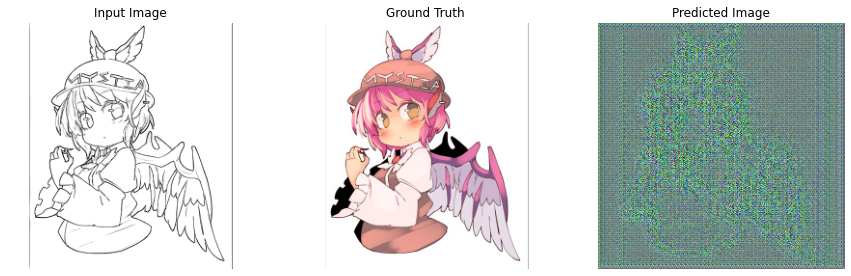
\includegraphics[scale = 0.35]{0ep.png}
        \caption{Result : 0 epochs}
    \end{figure}
\end{frame}
\begin{frame}{Image Translation Using GANs -- Results}
     \begin{figure}[h]
        \centering
        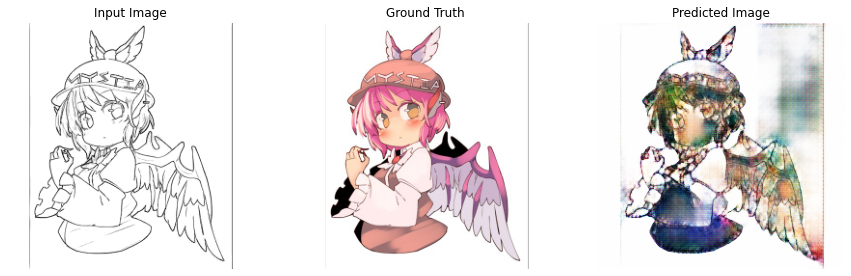
\includegraphics[scale = 0.35]{20ep.png}
        \caption{Result : 20 epochs}
    \end{figure}
\end{frame}
\begin{frame}{Image Translation Using GANs -- Results}
     \begin{figure}[h]
        \centering
        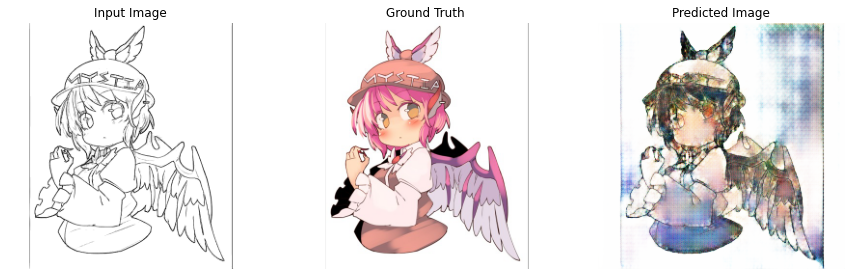
\includegraphics[scale = 0.35]{40ep.png}
        \caption{Result : 40 epochs}
    \end{figure}
\end{frame}
\begin{frame}{Image Translation Using GANs -- Results}
     \begin{figure}[h]
        \centering
        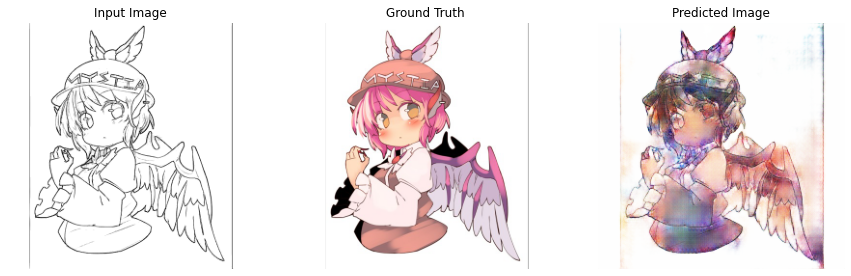
\includegraphics[scale = 0.35]{60ep.png}
        \caption{Result : 60 epochs}
    \end{figure}
\end{frame}

\section{Contribution and Code Sources}
\begin{frame}{Contribution}
    \begin{itemize}
        \item Siddhant Midha (200070078) 
        \begin{enumerate}
            \item Theory part of report
            \item Presentation slides
            \item Wrote code and trained for basicGAN
            \item Wrote code and trained for convGAN
            \item Modified the convGAN code to form condGAN and trained
        \end{enumerate}
         \item Waqar Mirza (200070090)
        \begin{enumerate}
            \item Results part of report.
            \item Trained the Anime Colourization GAN.
            \item Presentation slides - Image Translation using GANs
        \end{enumerate}
         \item Dadhichi Telwadkar (20D070083)
        \begin{enumerate}
            \item Code for Anime Colourization GAN.
        \end{enumerate}
         \item Yuvraj Singh (200070093)
        \begin{enumerate}
            \item Code for Anime Colourization GAN.
        \end{enumerate}
        
        
    \end{itemize}
\end{frame}
\begin{frame}{Code Sources}
    \begin{itemize}
        \item Referred to the GAN course on coursera for basic GAN theory and code organization.  
        \item Referred to the \texttt{Gradient Tape} and GAN tutorials by keras. 
        \item (None of the sources above involved direct use of code.)
        \item Referred to \href{https://towardsdatascience.com/generative-adversarial-networks-gans-89ef35a60b69}{this} tutorial for the Anime Colourization.
    \end{itemize}
\end{frame}
\end{document}
